\documentclass[14pt]{extarticle}
\usepackage{fontspec}
\usepackage{polyglossia}
\usepackage{amsmath}
\usepackage{amssymb}
\usepackage{xcolor}
\usepackage{fancyhdr}
\usepackage{graphicx}
\usepackage{listings}
\usepackage[most]{tcolorbox}
% \usepackage{setspace}
\usepackage{pifont}
\usepackage{enumitem}
\usepackage{titlesec}
\usepackage[bottom]{footmisc}
\usepackage{titling}
\usepackage{minted}
\usepackage{etoolbox}
\usepackage{array}
\usepackage{extsizes}
\usepackage{float}
\usepackage{booktabs}
\usepackage{hyperref}
\usepackage[onehalfspacing]{setspace}
\usepackage[a4paper, top=2.7cm, bottom=2.7cm, left=2.5cm, right=2.5cm, headheight=1.5cm, headsep=0.5cm]{geometry}
\usepackage{tikz}

\usetikzlibrary{automata, positioning, arrows.meta, arrows}

\newfontfamily\emoji{Segoe UI Emoji}

\pagestyle{fancy}

\setmainlanguage[numerals=western]{arabic}
\setotherlanguage{english}
% \newfontfamily\arabicfont[Script=Arabic]{Amiri}
\newfontfamily\arabicfont[Script=Arabic]{Calibri}
\newfontfamily\arabicfonttt[Script=Arabic]{Courier New}

\lstset{
  language=[Sharp]C,
  numbers=left,
  stepnumber=1,
  numbersep=8pt,
  frame=single,
  basicstyle=\ttfamily\small,
  keywordstyle=\color{blue},
  stringstyle=\color{red},
  commentstyle=\color{green!50!black}
}

\newif\ifdetailed
\ifdefined\setdetailed
  \setdetailed
\fi

\newif\ifwithsols
\ifdefined\setwithsols
  \setwithsols
\fi

% unified tcolorboxes for articles
\tcbset{colback=white, colframe=black, fonttitle=\bfseries, boxrule=0.8pt}
\newtcolorbox{boxDef}[1][]{colback=blue!5!white,colframe=blue!75!black,
  title={{\emoji📘} تعريف\ifx\\#1\\\else ~#1\fi :}}
\newtcolorbox{boxExercise}[1][]{colback=cyan!5!white,colframe=cyan!70!black,
  title={{\emoji🧩} تمرين\ifx\\#1\\\else ~#1\fi :}}
\newtcolorbox{boxExample}[1][]{colback=yellow!5!white,colframe=orange!90!black,
  title={{\emoji📝} مثال\ifx\\#1\\\else ~#1\fi :}}
\newtcolorbox{boxNote}[1][]{colback=gray!10!white,colframe=black,
  title={{\emoji✨} ملاحظة\ifx\\#1\\\else ~#1\fi :}}
\newtcolorbox{boxAttention}[1][]{colback=magenta!10!white,colframe=magenta!80!black,
  title={{\emoji🔔} تنبيه\ifx\\#1\\\else ~#1\fi :}}
\newtcolorbox{boxWarning}[1][]{colback=red!5!white,colframe=red!75!black,
  title={{\emoji⚡} ملاحظة هامة\ifx\\#1\\\else ~#1\fi :}}
\newtcolorbox{boxSolution}[1][]{colback=green!5!white,colframe=green!60!black,
  title={{\emoji✅} حل\ifx\\#1\\\else ~#1\fi :}}
\newtcolorbox{boxSymbol}[1][]{colback=purple!5!white,colframe=purple!70!black,
  title={{\emoji🔣} رمز\ifx\\#1\\\else ~#1\fi :}}
\newtcolorbox{boxHint}[1][]{colback=teal!5!white,colframe=teal!60!black,
  title={{\emoji💡} تلميح\ifx\\#1\\\else ~#1\fi :}}


\tcbset{simplecode/.style={ colback=gray!5, colframe=black!50, boxrule=0.4pt, arc=2pt, left=4pt,right=4pt,top=4pt,bottom=4pt}}
\newenvironment{boxCode}{\begin{tcolorbox}[simplecode]}{\end{tcolorbox}}

\newcolumntype{C}[1]{>{\centering\arraybackslash}p{#1}}

% redefine spaces after titles
\makeatletter
\renewcommand{\@maketitle}{%
  \begin{center}
    {\huge \bfseries \@title \par}%
    \vskip 0.2em % space between title and author
    {\large \@author \par}%
    % \vskip 0.2em % space between author and date
    % {\normalsize \@date \par}%
  \end{center}
}
\makeatother

\fancyhf{} % clear default
\fancypagestyle{plain}{
  \fancyhf{}
  \fancyhead[L]{مدرسة التسامح الشاملة}
  % \fancyhead[L]{
\includegraphics[height=1cm]{../../../images/logoTasamoh.png}}
  \fancyhead[R]{الأستاذ محمود اغبارية}
  \fancyfoot[C]{\thepage}
}

\fancyhead[L]{مدرسة التسامح الشاملة}
\fancyhead[R]{الأستاذ محمود اغبارية}
\fancyfoot[C]{\thepage}
% \date{\today}

\setcounter{tocdepth}{3} % only section subsection and subsubsection in TOC

\newcommand{\importpdfpage}[2]{%
    \thispagestyle{empty}
    \newgeometry{left=0cm,right=0cm,top=0cm,bottom=0cm}
    \includegraphics[page=#2,width=0.95\paperwidth,height=0.95\paperheight,keepaspectratio]{#1}
    \restoregeometry
}

\newcommand{\insertFullImg}[1]{%
    \noindent
    \makebox[\textwidth][c]{
        \includegraphics[width=0.9\paperwidth,keepaspectratio]{#1}%
    }%
}%

% ----------------------


% \begin{document}

% \maketitle

% % \clearpage  % start TOC on a new page
% % \renewcommand{\contentsname}{جدول المحتويات}
% % \tableofcontents
% % \clearpage

% \part*{part 1} % the * prevents numbering
% \section*{مقدمة}
% \subsection*{مثال رياضي}
% \subsubsection*{مثال فرعي}
% \paragraph*{ paragraph 1}
% \subparagraph*{sub paragraph 1}

% \ifdetailed
% \begin{english}
% \begin{minted}{csharp}
% // C# Example
% \end{minted}
% \end{english}
% \fi

% OLD WAY
% \ifdetailed
% \begin{english}
% \begin{lstlisting}
% // C# Example
% \end{lstlisting}
% \end{english}
% \fi

% % 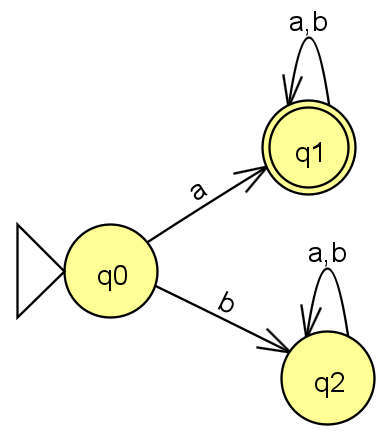
\includegraphics[width=0.2\textwidth]{../../../images/DFAs/ex1_q1.png}



% \vspace{3cm}
% \begin{flushleft}
% أرجو لكم وقتًا ممتعًا.

% الأستاذ محمود اغبارية.
% \end{flushleft}


% \end{document}


\ifwithsols
\title{حل ورقة تمرّن 10 - الحلقات المتداخلة \\ تحضير لترتيب الإدخال}
\else
\title{ورقة تمرّن 10 - الحلقات المتداخلة \\ تحضير لترتيب الإدخال}
\fi

\begin{document}

\maketitle
\thispagestyle{fancy}

\begin{enumerate}[itemsep=2em]
    \item
    اكتب عملية خارجية \textenglish{InsertAt} تتلقى مصفوفة أعداد صحيحة \textenglish{arr}، عدداً صحيحاً \textenglish{val}، ومؤشراً \textenglish{idx}. \\
    تقوم العملية بـ \textbf{إزاحة} جميع العناصر بدءاً من المؤشر \textenglish{idx} خطوة واحدة إلى اليمين (مما يؤدي إلى مسح العنصر الأخير في المصفوفة واستبداله)، ثم تضع العدد \textenglish{val} في الخانة \textenglish{idx}.

    \begin{boxExample}
    \begin{itemize}
        \item المصفوفة قبل الاستدعاء: \textenglish{\{10, 20, 30, 40, 50\}}، العدد \textenglish{val = 99}، والمؤشر \textenglish{idx = 2}.
        \item بعد استدعاء العملية تصبح: \textenglish{\{10, 20, \textbf{99}, 30, 40\}}.
    \end{itemize}
    \end{boxExample}

    \ifwithsols
    \begin{boxSolution}
    \begin{english}
    \begin{minted}{csharp}
public static void InsertAt(int[] arr, int val, int idx)
{
    for(int i = arr.Length - 2; i >= idx; i--)
    {
        arr[i + 1] = arr[i];
    }
    arr[idx] = val;
}
    \end{minted}
    \end{english}
    \end{boxSolution}
    \clearpage
    \fi

    \item
    نفس السؤال السابق، لكن العملية لا تتلقى المؤشر \textenglish{idx}، بل تتلقى مصفوفةً مرتبة تصاعديًّا وعدداً صحيحاً \textenglish{val} فقط \\
    على العملية أن تجد المكان الصحيح لإدراج هذا العدد في المصفوفة بحيث تبقى المصفوفة مرتبة تصاعديًّا. \\
    الحد الأخير في المصفوفة الأصلية سيحذف.

    \begin{boxExample}
    \begin{itemize}
        \item المصفوفة قبل الاستدعاء: \textenglish{\{10, 20, 30, 40, 50\}}، العدد \textenglish{val = 25}.
        \item بعد استدعاء العملية تصبح: \textenglish{\{10, 20, \textbf{25}, 30, 40\}}.
    \end{itemize}
    \end{boxExample}

    \begin{boxHint}
     اتبع نفس الخطوات السابقة، لكن بدلاً من تلقي المؤشر \textenglish{idx}، ابحث عن المكان الصحيح له أولاً من خلال حلقة، ثم قم بعملية الإزاحة والإدراج.
     \end{boxHint}

    \ifwithsols
    \begin{boxSolution}
    \begin{english}
    \begin{minted}{csharp}
public static void InsertInSortedArray(int[] arr, int val)
{
    int idx = 0;
    while (idx < arr.Length && arr[idx] < val)
    {
        idx++;
    }
    for(int i = arr.Length - 2; i >= idx; i--)
    {
        arr[i + 1] = arr[i];
    }
    arr[idx] = val;
}
    \end{minted}
    \end{english}
    \end{boxSolution}
    \fi

    \clearpage
\item
    معطاة مصفوفة أعداد صحيحة \textenglish{arr}، جميع عناصرها \textbf{مرتبة تصاعدياً} ما عدا \textbf{العنصر الأخير} الذي تمت إضافته للتو وقد يكون في المكان الخاطئ. \\
    اكتب عملية خارجية \textenglish{SortLastItem} تتلقى هذه المصفوفة، وتقوم بإدراج هذا العنصر الأخير في مكانه الصحيح بحيث تصبح المصفوفة بأكملها مرتبة.

    \begin{boxExample}
    \begin{itemize}
        \item المصفوفة قبل الاستدعاء: \textenglish{\{3, 7, 10, 15, \textbf{6}\}} (الرقم 6 ليس في مكانه).
        \item بعد استدعاء العملية تصبح: \textenglish{\{3, \textbf{6}, 7, 10, 15\}}.
    \end{itemize}
\end{boxExample}

    \begin{boxHint}
    \begin{enumerate}
        \item احفظ قيمة العنصر الأخير في متغير مساعد.
        \item ابحث عن الخانة (الإندكس) الصحيحة التي يجب أن يوضع فيها هذا العنصر.
        \item قم بإزاحة جميع العناصر الأكبر منه خطوة واحدة إلى اليمين لتفريغ مكان له.
        \item ضع العنصر في مكانه الصحيح.
    \end{enumerate}
\end{boxHint}


    \ifwithsols
    \begin{boxSolution}[1]
    \begin{english}
    \begin{minted}{csharp}
public static void SortLastItem(int[] arr)
{
    int tmp = arr[arr.Length - 1];
    int idx = 0;
    while (idx < arr.Length && arr[idx] < tmp)
    {
        idx++;
    }
    for(int i = arr.Length - 2; i >= idx; i--)
    {
        arr[i + 1] = arr[i];
    }
    arr[idx] = tmp;
}
    \end{minted}
    \end{english}
    \end{boxSolution}
    % \clearpage
    \begin{boxSolution}[2]
    \begin{english}
    \begin{minted}{csharp}
public static void SortLastItem(int[] arr)
{
    int tmp = arr[arr.Length-1];
    int idx = arr.Length - 2;
    while (idx >= 0 && arr[idx] > tmp)
    {
        arr[idx + 1] = arr[idx];
        idx--;
    }
    arr[idx + 1] = tmp;
}
    \end{minted}
    \end{english}
    \end{boxSolution}
    \fi

\end{enumerate}

\end{document}
